\begin{figure}[t]
\centering
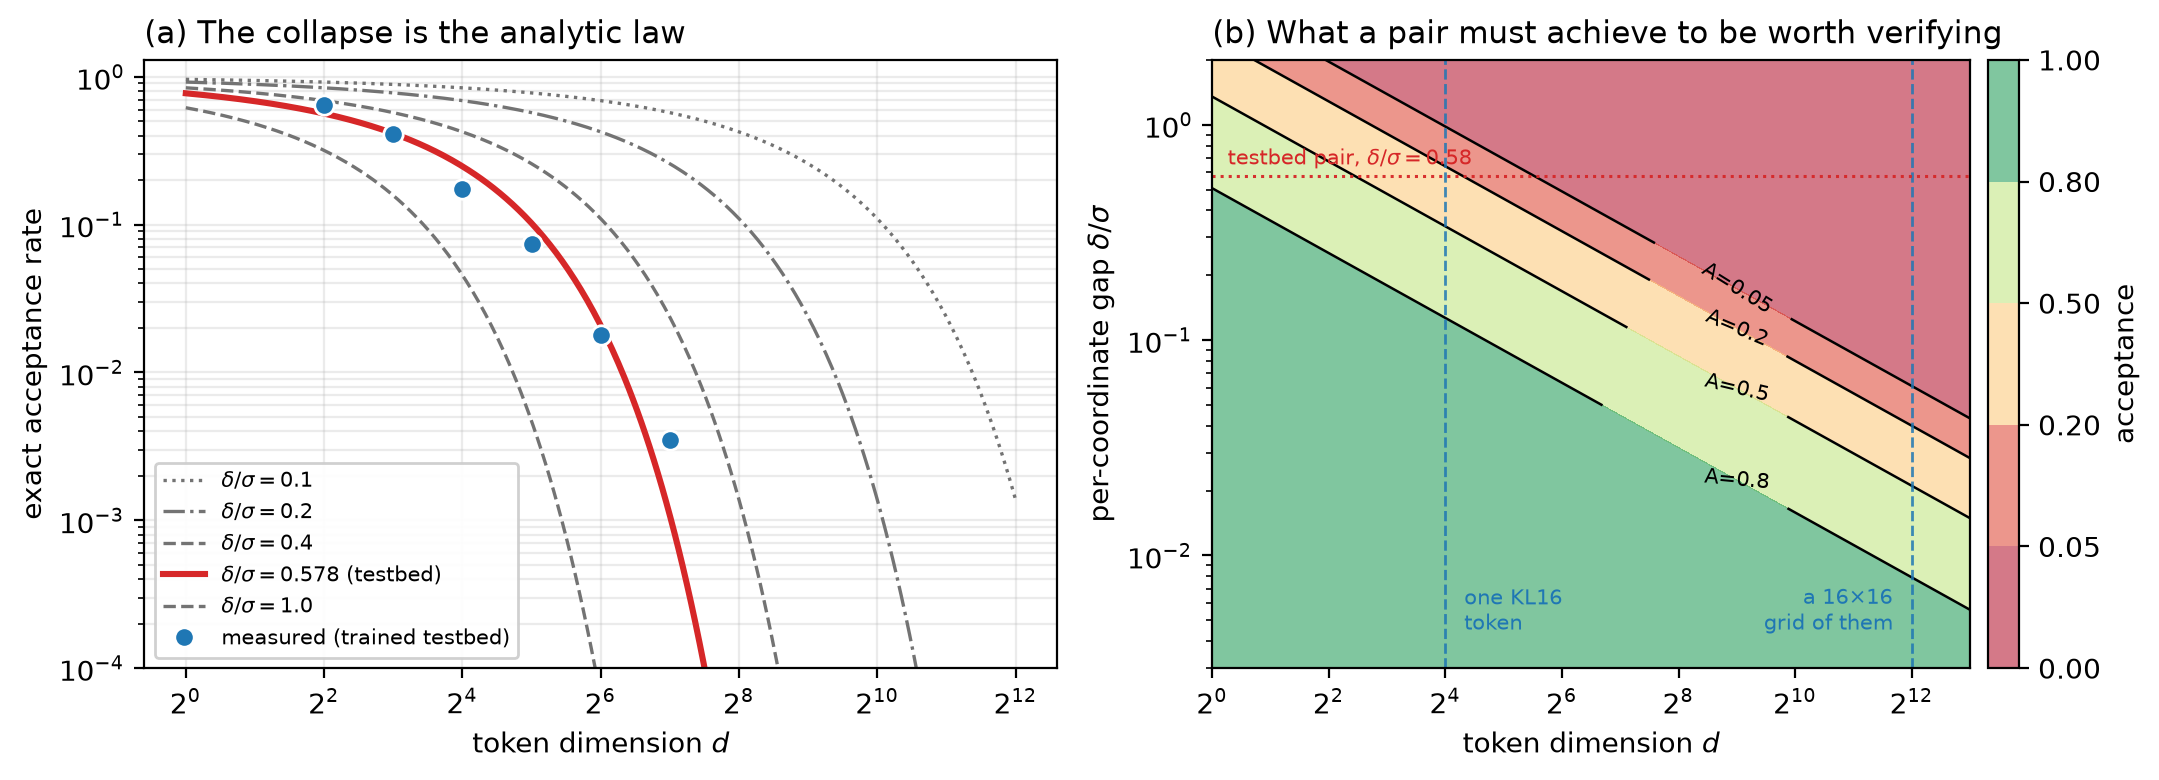
\includegraphics[width=0.86\textwidth]{figures/e08_feasibility.png}
\caption{\textbf{The collapse is an analytic law, and it has an engineering reading.}
\textbf{(a)} Exact acceptance against token dimension for shared-covariance Gaussians at several
fixed per-coordinate gaps, with the trained testbed's six measured rates overlaid. The measurements
track the $\delta/\sigma = 0.578$ curve they should, so the sweep samples a law rather than an
artefact of one architecture, and the law continues past the widths we can train: at $\dd = 256$
acceptance is already below $10^{-5}$. \textbf{(b)} The same statement as a design constraint.
Contours of acceptance over token dimension and per-coordinate disagreement are lines of
$\delta\sqrt{\dd} = \text{const}$, so on log--log axes they have slope $-1/2$ and every doubling of
the token width costs a factor $\sqrt2$ in the agreement a pair must reach. One KL16 token
($\dd{=}16$) tolerates a gap of $0.34\sigma$ at acceptance $0.5$; the $16\times16$ grid of them that
makes up an image ($\dd{=}4096$) tolerates $0.021\sigma$.}
\label{fig:feasibility}
\end{figure}
